%!TEX root = reparam_nips2016.tex
\vspace*{-6pt}
\section{Experiments}
\vspace*{-5pt}
We apply \gls{G-REP} to perform mean-field \gls{VI} on two nonconjugate probabilistic models: the sparse gamma \gls{DEF} and a beta-gamma \gls{MF} model.
%
The sparse gamma \gls{DEF} \citep{Ranganath2015} is a probabilistic model with several layers of latent locations and latent weights, mimicking the architecture of a deep neural network. The weights of the model are denoted by $w_{k k^\prime}^{(\ell)}$, where $k$ and $k^\prime$ run over latent components, and $\ell$ indexes the layer. The latent locations are $z_{nk}^{(\ell)}$, where $n$ denotes the observation. We consider Poisson-distributed observations $x_{nd}$ for each dimension $d$. Thus, the model is specified as
\vspace*{-2pt}
\begin{align}
    & z_{nk}^{(\ell)} \sim \textrm{Gamma}\left(\alpha_z, \frac{\alpha_z}{\sum_{k^\prime} z_{nk^\prime}^{(\ell+1)} w_{k^\prime k}^{(\ell)}}\right),\qquad
    x_{nd} \sim \textrm{Poisson}\left(\sum_{k^\prime} z_{nk^\prime}^{(1)} w_{k^\prime d}^{(0)}\right).\nonumber
\end{align} \vspace*{-2pt}%
We place gamma priors over the weights $w_{k k^\prime}^{\ell}$ with rate $0.3$ and shape $0.1$, and a gamma prior with rate $0.1$ and shape $0.1$ over the top-layer latent variables $z_{nk}^{(L)}$. We set the hyperparameter $\alpha_z=0.1$, and we use $L=3$ layers with $100$, $40$, and $15$ latent factors.

The second model is a beta-gamma \gls{MF} model with weights $w_{kd}$ and latent locations $z_{nk}$. We use this model to describe binary observations $x_{nd}$, which are modeled as
\vspace*{-2pt}
\begin{equation}\nonumber
    x_{nd} \sim \textrm{Bernoulli}\left(\sigmoid{\sum_{k} \logit{z_{nk}} w_{kd}}\right),
\end{equation} \vspace*{-2pt}%
where $\logit{z}=\log(z/(1-z))$ and $\sigmoid{\cdot}$ is the inverse logit function. We place a gamma prior with shape $0.1$ and rate $0.3$ over the weights $w_{kd}$, a uniform prior over the variables $z_{nk}$, and we use $K=100$ latent components.

\parhead{Datasets.}
We apply the sparse gamma \gls{DEF} on two different databases: (i) the Olivetti database at AT\&T,\footnote{\url{http://www.cl.cam.ac.uk/research/dtg/attarchive/facedatabase.html}} which consists of 400 (320 for training and 80 for test) $64\times 64$ images of human faces in a 8 bit scale ($0-255$); and (ii) the collection of papers at the Neural Information Processing Systems (\textsc{nips}) 2011 conference, which consists of $305$ documents and a vocabulary of $5715$ effective words in a bag-of-words format ($25\%$ of words from all documents are set aside to form the test set).

We apply the beta-gamma \gls{MF} on: (i) the binarized \textsc{mnist} data,\footnote{\url{http://yann.lecun.com/exdb/mnist}} which consists of $28\times 28$ images of hand-written digits (we use $5000$ training and $2000$ test images); and (ii) the Omniglot dataset \citep{Lake2015}, which consists of $105\times 105$ images of hand-written characters from different alphabets (we select 10 alphabets, with $4425$ training images, $1475$ test images, and $295$ characters).

\vspace*{-1pt}
\parhead{Evaluation.}
We apply mean-field \gls{VI} and we compare \gls{G-REP} with \gls{BBVI} \citep{Ranganath2014} and \gls{ADVI} \citep{Kucukelbir2016}. We do not apply \gls{BBVI} on the Omniglot dataset due to its computational complexity.
%
At each iteration, we evaluate the \gls{ELBO} using one sample from the variational distribution, except for \gls{ADVI}, for which we use $20$ samples (for the Omniglot dataset, we only use one sample). We run each algorithm with a fixed computational budget of CPU time. After that time, we also evaluate the predictive log-likelihood on the test set, averaging over 100 posterior samples. For the \textsc{nips} data, we also compute the test perplexity (with one posterior sample) every 10 iterations, given by
\vspace*{-2pt}
\begin{equation}\nonumber
  \exp\left(\frac{-\sum_{\rm docs}\sum_{w\in \textrm{doc}(d)} \log p(w\g \#\textrm{held out in doc}(d))}{\# \textrm{held out words}}\right).
\end{equation}

\vspace*{-7pt}
\parhead{Experimental setup.}
To estimate the gradient, we use $30$ Monte Carlo samples for \gls{BBVI}, and only $1$ for \gls{ADVI} and \acrshort{G-REP}. For \gls{BBVI}, we use Rao-Blackwellization and control variates (we use a separate set of $30$ samples to estimate the control variates). For \gls{BBVI} and \acrshort{G-REP}, we use beta and gamma variational distributions, whereas \gls{ADVI} uses Gaussian distributions on the transformed space, which correspond to log-normal or logit-normal distributions on the original space. Thus, only \acrshort{G-REP} and \gls{BBVI} optimize the same variational family. We parameterize the gamma distribution in terms of its shape and mean, and the beta in terms of its shape parameters $\alpha$ and $\beta$. To avoid constrained optimization, we apply the transformation $v^\prime=\log(\exp(v)-1)$ to the variational parameters that are constrained to be positive and take stochastic gradient steps with respect to $v^\prime$. We use the analytic gradient of the entropy terms. We implement \gls{ADVI} as described by \citet{Kucukelbir2016}.

We use the step-size schedule in Eq.~\ref{eq:step_schedule}, and we explore the parameter $\eta\in\{0.1,0.5,1,5\}$. For each algorithm and each dataset, we report the results based on the value of $\eta$ for which the best \gls{ELBO} was achieved. We report the values of $\eta$ in Table~\ref{tab:eta_and_runtime} (left).


% \begin{table}[t]
%   \small
%   \centering
%   \begin{tabular}{crlrlrlrlrl}\toprule
%       & \multicolumn{2}{c}{Olivetti} & \multicolumn{2}{c}{\textsc{nips}} & \multicolumn{2}{c}{\textsc{mnist(5k)}} & \multicolumn{2}{c}{\textsc{mnist(50k)}} & \multicolumn{2}{c}{Omniglot} \\ \hline
%       \acrshort{G-REP} & $5$ & $0.46$ & $0.5$ & $0.83$ & $5$ & $1.09$ & $5$ & $8.08$ & $5$ & $5.50$ \\
%       \acrshort{BBVI} & $1$ & $12.90$ & $5$ & $20.95$ & $5$ & $25.99$ & $-$ & $-$ & $-$ & $-$ \\
%       \acrshort{ADVI} & $0.1$ & $0.17$ & $1$ & $0.25$ & $0.1$ & $0.34$ & $0.5$ & $2.04$ & $0.1$ & $4.10$ \\ \bottomrule
%   \end{tabular}
%   \caption{\label{tab:eta_and_runtime}(Left) Step-size constant $\eta$, reported for completeness. (Right) Average time per iteration in seconds. \acrshort{G-REP} is $1$-$4$ times slower than \gls{ADVI} but above one order of magnitude faster than \gls{BBVI}.}
%   \vspace*{-9pt}
% \end{table}

\begin{table}[t]
  \small
  \centering
  \begin{tabular}{cccc}\toprule
     \textbf{Dataset} & \acrshort{G-REP} & \gls{BBVI} & \gls{ADVI} \\ \hline
     Olivetti & $5$ & $1$ & $0.1$ \\ 
     \textsc{nips} & $0.5$ & $5$ & $1$ \\ 
     \textsc{mnist} & $5$ & $5$ & $0.1$ \\ 
     Omniglot & $5$ & $-$ & $0.1$ \\ \bottomrule
  \end{tabular}
  \hspace*{30pt}
  \begin{tabular}{cccc}\toprule
     \textbf{Dataset} & \acrshort{G-REP} & \gls{BBVI} & \gls{ADVI} \\ \hline
     Olivetti     & $0.46$  & $12.90$ & $0.17$ \\ 
     \textsc{nips}  & $0.83$  & $20.95$ & $0.25$ \\ 
     \textsc{mnist} & $1.09$  & $25.99$ & $0.34$ \\ 
     Omniglot     & $5.50$  & $-$   & $4.10$ \\ \bottomrule
  \end{tabular}
  \caption{\label{tab:eta_and_runtime}(Left) Step-size constant $\eta$, reported for completeness. (Right) Average time per iteration in seconds. \acrshort{G-REP} is $1$-$4$ times slower than \gls{ADVI} but above one order of magnitude faster than \gls{BBVI}.}
  \vspace*{-9pt}
\end{table}

\vspace*{-1pt}
\parhead{Results.}
We show in Figure~\ref{fig:elbo} the evolution of the \gls{ELBO} as a function of the running time for three of the considered datasets. \gls{BBVI} converges slower than the rest of the methods, since each iteration involves drawing multiple samples and evaluating the log-joint for each of them. \gls{ADVI} and \acrshort{G-REP} achieve similar bounds, except for the \textsc{mnist} dataset, for which \acrshort{G-REP} provides a variational approximation that is closer to the posterior, since the \gls{ELBO} is higher. This is because a variational family with sparse gamma and beta distributions provides a better fit to the data than the variational family to which \gls{ADVI} is limited (log-normal and logit-normal). \gls{ADVI} seems to converge slower; however, we \emph{do not} claim that \gls{ADVI} converges slower than \acrshort{G-REP} in general. Instead, the difference may be due to the different step-sizes schedules that we found to be optimal (see Table~\ref{tab:eta_and_runtime}). We also report in Table~\ref{tab:eta_and_runtime} (right) the average time per iteration\footnote{%
	On the full \textsc{mnist} with $50,000$ training images, \acrshort{G-REP} (\acrshort{ADVI}) took $8.08$ ($2.04$) seconds per iteration.
} for each method: \gls{BBVI} is the slowest method, and \gls{ADVI} is the fastest because it involves simulation of Gaussian random variables only.

However, \acrshort{G-REP} provides higher likelihood values than \gls{ADVI}. We show in Figure~\ref{fig:pred_nips} the evolution of the perplexity (lower is better) for the \textsc{nips} dataset, and in Figure~\ref{tab:pred_llh} the resulting test log-likelihood (larger is better) for the rest of the considered datasets. In Figure~\ref{tab:pred_llh}, we report the mean and standard deviation over $100$ posterior samples. \gls{ADVI} cannot fit the data as well as \acrshort{G-REP} or \gls{BBVI} because it is constrained to log-normal and logit-normal variational distributions. These cannot capture sparsity, which is an important feature for the considered models. We can also conclude this by a simple visual inspection of the fitted models. In the Supplement, we compare images sampled from the \acrshort{G-REP} and the \gls{ADVI} posteriors, where we can observe that the latter are more blurry or lack some details.

\begin{figure}[t]
	\centering
	\subfloat[\gls{ELBO} (Olivetti dataset).\label{fig:elbo_faces}]{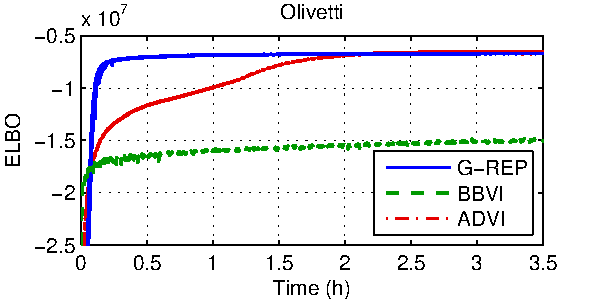
\includegraphics[width=0.34\textwidth]{figures/plt_faces.pdf}}\hspace*{-11pt}
	\subfloat[\gls{ELBO} (\textsc{mnist} dataset).\label{fig:elbo_bmnist}]{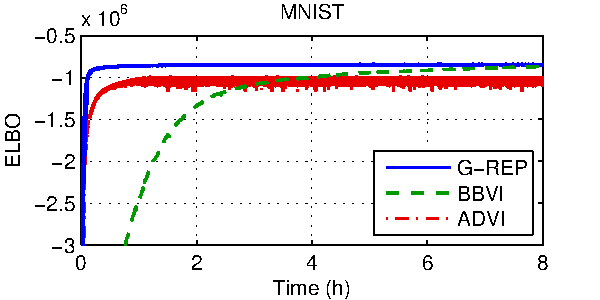
\includegraphics[width=0.34\textwidth]{figures/plt_bmnist5K.pdf}}\hspace*{-15pt}
	\subfloat[\gls{ELBO} (Omniglot dataset).\label{fig:elbo_omniglot}]{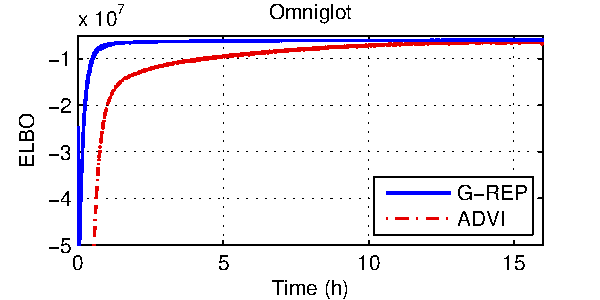
\includegraphics[width=0.34\textwidth]{figures/plt_omniglot10a.pdf}}
  \vspace*{-4pt}
	\caption{\label{fig:elbo}Comparison between \acrshort{G-REP}, \gls{BBVI}, and \gls{ADVI} in terms of the variational objective function.}
  \vspace*{-12pt}
\end{figure}

\begin{figure}[t]
  \centering
  \subfloat[Perplexity (\textsc{nips} dataset).\label{fig:pred_nips}]{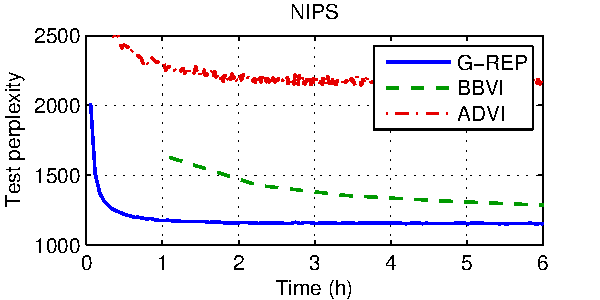
\includegraphics[width=0.34\textwidth]{figures/plt_nips.pdf}}
  \raisebox{27pt}{
    \subfloat[Average test log-likelihood per entry $x_{nd}$.\label{tab:pred_llh}]{%
      \small
      \setlength{\tabcolsep}{2.5pt}
      \begin{tabular}{cccc}\toprule
         \textbf{Dataset} & \acrshort{G-REP} & \gls{BBVI} & \gls{ADVI} \\ \hline
         Olivetti & $\mathbf{-4.48\pm 0.01}$ & $-9.74\pm 0.08$ & $-4.63\pm 0.01$ \\ 
         \textsc{mnist} & $-0.0932\pm 0.0004$ & $\mathbf{-0.0888\pm 0.0004}$ & $-0.189\pm 0.009$ \\ 
         Omniglot & $\mathbf{-0.0472\pm 0.0001}$ & $-$ & $-0.0823\pm 0.0009$ \\ \bottomrule
      \end{tabular}
    }
  }
  \vspace*{-4pt}
  \caption{\label{fig:pred_perm}Comparison between \acrshort{G-REP}, \gls{BBVI}, and \gls{ADVI} in terms of performance on the test set. \acrshort{G-REP} outperforms \gls{BBVI} because the latter has not converged in the allowed time, and it also outperforms \gls{ADVI} because of the variational family it uses.}
  \vspace*{-4pt}
\end{figure}


